\chapter{Implementatie}
In het vorige hoofdstuk is er beschreven hoe de architectuur van een monitoring library eruit kan zien. In dit hoofdstuk wordt er gekeken naar de implementatie van de Tracklytics library. %\cite{tracklytics}
Er wordt gekeken naar welke technologie\"en er gebruikt zijn bij het ontwikkelen van de library. Daarnaast wordt er uitgelegd hoe developers de library kunnen gebruiken in hun applicaties. Er wordt dieper ingegaan op de communicatie tussen de Tracklytics library en de server.

\section{Details Implementatie}
In deze sectie wordt er besproken welke technologie\"en er gebruikt zijn bij het ontwikkelen van de Tracklytics library.

\subsection{iOS Library}
De Tracklytics library beschreven in deze thesis is ontwikkeld voor het iOS besturingssysteem. Voor het iOS besturingssysteem bestaan er twee programmeertalen om een applicatie, of in dit geval een library, te ontwikkelen, namelijk: Swift en Objective-C. Swift is een redelijk recente taal, op het moment van schrijven is deze nog geen twee jaar oud. Omdat de ondersteuning van Swift door de meerderheid van de developers nog zeer karig is, is er besloten om de library in Objective-C te schrijven. Objective-C en Swift hebben dezelfde functionaliteiten, maar programmeren in Swift is overzichtelijker door de andere syntax. Swift is meer ge\"integreerd in de IDE die Apple aanbiedt om applicaties mee te ontwikkelen. Swift is veiliger en sneller dan Objective-C. Al deze redenen pleiten om Swift als programmeertaal te kiezen. Het grote nadeel is dat Swift nog niet in veel applicaties aanwezig is en dat het moeilijker is om in een Swift applicatie een Objective-C library te integreren dan andersom. Dit is de grote reden waarom er voor Objective-C gekozen is.\\
%cite swift

De Tracklytics library slaat tijdelijk de data op op de harde schijf van het toestel. Dit heeft twee voordelen, namelijk: er gaat geen data verloren en de library gebruikt minder RAM.
Als het toestel geen internet connectie zou hebben, kan de library de data niet verzenden naar de back end en indien de applicatie dan sluit zijn alle gegevens verloren. Dit scenario is opgelost door het tijdelijk opslaan van de gegevens op de harde schijf. De data wordt pas verwijderd als de library er zeker van is dat de data succesvol naar de back end is verstuurd. 

Een mobiel toestel heeft een beperkte grootte RAM geheugen en applicaties kunnen hier niet volledig gebruik van maken omdat het besturingssysteem dit geheugen ook gebruikt. Als de applicatie teveel RAM geheugen gebruikt, dan gaat heel de applicatie deze trager werken, omdat het RAM geheugen dan uitgeswapt wordt naar de harde schijf. Het is dus noodzakelijk om het RAM gebruik zo laag mogelijk te houden. Indien alle data in RAM geheugen zou gehouden gestoken worden, dan kan dit snel vollopen. Het opslaan van de data op de harde schijf verhelpt dit probleem. Het is dan wel noodzakelijk dat het opslaan van de data op schijf in de achtergrond gebeurt, omdat I/O operaties relatief lang duren. \\

De methodes van de Tracklytics library die gebruikt kunnen worden zijn statische methodes. De keuze hiervoor is gebaseerd op twee redenen.

De Tracklytics library klasse die de methodes aanbiedt is geen objectgerichte klasse. Indien er een object van deze klasse zou gemaakt worden, zou deze elke keer na creatie bijna onmiddelijk niet meer gebruikt worden. Deze creatie van het object zorgt voor een overhead, de welke is weggewerkt door het statisch maken van alle methodes die bruikbaar zijn door de developers. 

Een tweede reden is de gebruiksvriendelijkheid. Een library call neemt maar \'e\'en lijn code in om een methode uit te voeren in plaats van twee. Dit zorgt voor minder code. De impact hiervan hangt af van het aantal monitoring punten die in de applicatie zijn ingevoerd. Dit verbetert ook de leesbaarheid van de code.\\

\subsection{Back end}
De data die de Tracklytics library doorstuurt vanaf het toestel van de gebruiker moet opgeslagen worden in een database. Zo kan deze data later verwerkt worden en worden weergegeven in het dashboard. Er moet een keuze gemaakt worden over het besturingssysteem, de database en de programmeertaal van de back end.\\

De server draait in OpenStack, een cloud platform. Deze is gedeployed als infrastructure-as-a-service (IaaS). Dit wil zeggen dat dit meerdere virtuele servers kan aanbieden (zelfs meerdere virtuele servers als fysieke servers). Dit biedt een abstractie en schermt de virtuele server af van andere virtuele servers. Een gebruiker kan zelf nieuwe virtuele servers aanmaken. Elke virtuele server heeft zijn eigen besturingssysteem, te kiezen uit een lijst van images aangeboden door OpenStack. 
%\cite openstack

In de Tracklytics architectuur is gekozen voor een linux distributie (in dit geval Ubuntu). Deze keuze is gemaakt op basis van de gebruiksvriendelijkheid van dit besturingssysteem. Zo is het gemakkelijk om snel een webserver op te zetten en een database te installeren. Er is voor Ubuntu gekozen, omdat dit de meest gekende en meest gebruikte linux distributie is. \\
%\cite ubuntu

In de database wordt alle data opgeslagen, wat wil zeggen dat dit een van de meest belangrijke onderdelen van de Tracklytics architectuur vormt. De metadata die gecollecteerd wordt per applicatie is in vele gevallen hetzelfde. De parameters die verschillen zijn: het type toestel, het type internet connectie en de versie van de applicatie. Dit gegeven zorgt ervoor dat de metadata vaak hetzelfde is. Indien de metadata uit de data komende van de Tracklytics library wordt uitgehaald kan er relatief veel opslagruimte gespaard worden, omdat deze metadata niet in elke entry in de database aanwezig moet zijn, enkel een verwijzing naar waar die metadata staat. Er is gekozen om een MySQL database te gebruiken, omdat deze een gestructureerde tabellenstructuur heeft en zo de metadata gemakkelijk van de data kan scheiden. De data kunnen door SQL queries gecombineerd worden in views om de data overzichtelijk te maken. Een alternatief is een NoSQL database. Dit alternatief past niet in de manier waarop de data opgeslagen wordt, omdat deze een niet-gestructureerde database aanbiedt. \\

De back end heeft in de Tracklytics library twee functies, namelijk: het verwerken en opslaan van de data in de database en het opvragen van data uit de database om het dashboard van de data te voorzien. De keuze is gevallen op PHP als programmeertaal. Met PHP is het simpel om een database connectie op te zetten en via SQL queries deze dat in of uit de database te krijgen. Een tweede voordeel van PHP is dat deze met POST data om kan. Via deze manier kan de data in de request van de Tracklytics library verborgen worden in de request en moet deze niet rechtstreeks doorgegeven worden in bijvoorbeeld de URL zelf. Zo is er meer veiligheid en privacy van de data. \\


\subsection{Dashboard}
Het Tracklytics dashboard is ontworpen om de gegevens van de applicatie in grafieken en details weer te geven om hieruit een conclusie te kunnen trekken over het functioneren van de applicatie. Het dashboard is ontworpen als webapplicatie in plaats van een desktop applicatie. De voordelen hiervan zijn: software updates automatisch worden doorgevoerd zonder dat er tussenkomst van de gebruiker nodig is, het is cross platform, omdat het in de browser draait en er is geen installatie vereist. \\

Om de webapplicatie te ontwikkelen is er gebruik gemaakt van AngularJS. De reden hiervoor is dat dit een zeer handig framework is voor het ontwikkelen van dynamische websites. Dit framework bindt stukken HTML code aan JavaScript code, wat ervoor zorgt dat het DOM gemakkelijk manipuleerbaar is door JavaScript. Een tweede reden waarom AngularJS in deze situatie voordelig is, is dat met AngularJS het gemakkelijk is om stukken HTML te laten herhalen met andere gegevens in. Zo kunnen de verschillende grafieken onder elkaar geplaatst worden zonder telkens de HTML code in JavaScript aan te moeten passen. Een bijkomstig voordeel is dat de data in de verschillende tabbladen maar eenmalig ingeladen moet worden, omdat AngularJS ervoor zorgt dat als je op een tab drukt niet de hele webpagina opnieuw wordt ingeladen, maar enkel de view die verandert ingeladen wordt.
%/cite angularJS

Om de grafieken weer te kunnen geven is ervoor gekozen om Chart.js (voor AngularJS) te gebruiken. Dit framework neemt data die in AngularJS variabelen gezet worden en geeft deze weer in een gekozen grafiek (bv. lijn-grafiek of staafdiagram). Chart.js is een simpele manier om snel een grafiek weer te kunnen geven, het werkt out-of-the-box en er zijn een aantal zeer handige opties die kunnen aangepast worden. 
%/cite Chart.js

De data die nodig is om de titels en de gegevens voor de grafieken in te laden moet uit de backend gehaald worden. Deze is zoals in vorige sectie aangehaald geschreven in PHP. De data wordt via AngularJS opgehaald en aan de juiste variabelen gekoppeld die ervoor zorgen dat deze data correct kan worden weergegeven.\\ 

\subsection{Connectie tussen Front end en Back end}
Zoals eerder aangegeven stuurt de front end (de Tracklytics iOS library) data naar de back end over een internetverbinding. Om ervoor te zorgen dat deze data veilig overgedragen wordt is ervoor gekomen om een HTTPS verbinding te gebruiken. Dit zorgt er automatisch voor dat er een veilige verbinding tussen client en server is. Een alternatief is de data zelf encoderen aan de client zijde en decoderen aan de server zijde. Omdat HTTPS ervoor zorgt dat de data veilig wordt overgedragen is ervoor gekozen om encoderen en decoderen niet te gebruiken.
Een andere beveligingskeuze die er is gemaakt is om HTTP POST te gebruiken in plaats van HTTP GET. HTTP POST verbergt de data in de request, terwijl HTTP GET de data in de URL van de request zet. De consequenties hiervan zijn dat de data in HTTP POST requests in geen enkele log of geschiedenis voorkomen, wat wel kan gebeuren met HTTP GET requests. Het is ook moeilijker de data in de HTTP POST requests aan te passen dan die van de HTTP GET requests, omdat het gemakkelijker is om een URL aan te passen dan een request zelf.\\

\section{Klassediagram} \label{sec:Klassediagram}
\begin{figure}[!h]
  \centering
  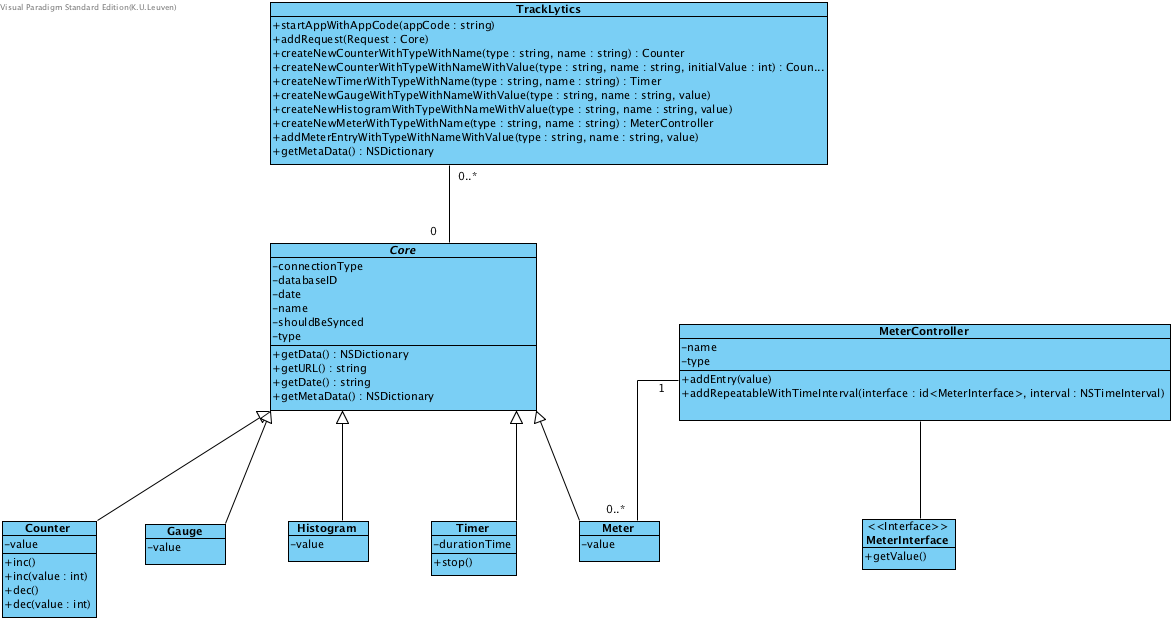
\includegraphics[scale=0.4]{Afbeeldingen/Implementatie/ClassDiagram}
  \caption{Klassediagram Tracklytics library.}
  \label{fig:fig}
\end{figure}

Het klassediagram duidt de klasses aan waaruit de Tracklytics libray bestaat. De verantwoordelijkheden van de verschillende klasses worden uitgelegd in de volgende secties.

\subsection{TrackLytics}
De Tracklytics klasse is de klasse die de synchronisatie met de server verzorgt. De klasse is ook verantwoordelijk voor het creëren en opslaan van de meetobjecten. De klasse heeft enkel statische methodes, dit zorgt ervoor dat de library gemakkelijker te gebruiken is omdat er geen object van deze klasse aangemaakt moet worden telkens de library gebruikt zou worden.

\subsection{Core}
Om de gemeenschappelijke elementen te combineren is ervoor gekozen om die gemeenschappelijke elementen in een abstracte superklasse te steken. De gemeenschappelijke methodes worden ook in de Core klasse gestoken, zodat de subklasses indien nodig dit kunnen overriden. 

\subsection{Counter}
De counter klasse stelt een telobject voor. Je kan bij een counter een getal optellen en aftrekken. De inc() functie verhoogt de value met 1 terwijl inc(x) de value verhoogt met x. Dit is opgesplitst omdat inc() vaker gebruikt gaat worden en zo moet er niet telkens inc(1) uitgevoerd worden. Hetzelfde geldt voor dec dat de value gaat verlagen. Deze functies zijn een onderdeel van de update call zoals besproken in vorige sectie \ref{sec:TrackingEnMonitoringVanGegevens}.

\subsection{Gauge}
De gauge klasse stelt een object met een waarde voor. Dit object wordt aangemaakt en opgeslagen met die waarde en gesynchroniseerd naar de server. Er zijn geen methodes beschikbaar speciaal voor dit object, omdat deze waarde niet aangepast zal worden.

\subsection{Histogram}
De gauge klasse en het histogram zijn maar op 1 punt verschillend en dat is in de back-end. De waarde van het histogram wordt ergens anders opgeslagen dan de waarde van de gauge. In de tracklytics library zijn ze dus hetzelfde, enkel de getUrl() methode geeft een andere url terug.

\subsection{Timer}
De timer klasse kan gebruikt worden om de duur van een gebeurtenis te meten. Bij het aanmaken van de timer wordt de huidige timestamp bijgehouden. De stop() methode neemt de huidige timestamp en vergelijkt die met degene die werd bijgehouden. Zo weten we de duur van de gebeurtenis. Indien de programmeur de methode stop() nooit aanroept wordt de timer niet gesynchroniseerd naar de server zodat er geen foute data tussen de data in de database staat. De stop() call is een onderdeel van de update call zoals besproken in vorige sectie \ref{sec:TrackingEnMonitoringVanGegevens}.

\subsection{Meter}
Een meter is bedoeld om een reeks van waarden te kunnen meten. Om dit voor de developer makkelijk te maken hebben we hiervoor 3 componenten uitgedacht: de Meter, de MeterController en de MeterInterface. De meter component is een uitzondering als er gekeken wordt naar het flow diagram uit de vorige sectie \ref{fig:flow2}. In plaats van dat een Meter object wordt terug gegeven, wordt er een MeterController object terug gegeven. Deze keuze is gemaakt, omdat het de structuur van de library versimpeld en het de developer gemakkelijker maakt.

\subsubsection{Meter}
Het meter object is het object dat opgeslagen wordt en dat gesynchroniseerd wordt naar de server. Het object houdt de value bij en ook het tijdstip van aanmaken.

\subsubsection{MeterController}
De metercontroller zorgt ervoor dat nieuwe meters aangemaakt kunnen worden. De metercontroller bevat de naam en het type van de meter. We kiezen ervoor om meters via deze weg aan te maken, omdat dit het werk van de programmeur vermindert. De programmeur moet enkel de waarde meegeven aan de metercontroller in plaats van telkens opnieuw de type en de naam mee te geven. We hebben het de programmeur nog op een manier gemakkelijk gemaakt. De metercontroller heeft de mogelijkheid om periodiek data op te halen van een functie die de programmeur specifiëert. Zo moet de programmeur dit niet zelf gaan doen in een bepaalde methode. 

\subsubsection{MeterInterface}
De meterinterface is de verbinding tussen de periodieke functie van de MeterController en het object waar de data op moet gehaald worden. Er is maar 1 functie, namelijk de getValue() die een waarde gaat ophalen. De programmeur vult deze methode dan in om de correcte waarde terug te geven.


